\chapter{Project Organisation}
 
\noindent \textbf{When will the team work together and what tools will it use to work outside meeting hours?}

\vspace{1em}
\noindent The team will work together every Wednesday and will use Facebook Messenger to communicate and Team Viewer to work at home. 

\vspace{1em}
\noindent \textbf{Who is the project coordinator and what is his role?}

\vspace{1em}
\noindent Mohammad Ali Syed will be the project coordinator and will be responsible for maintaining communication between all team members and organising the required deliverables and submitting them. 

\vspace{1em}
\noindent \textbf{How will the project be divided between team members?}

\begin{table}[h!]
\centering
\begin{tabular}{ |c|c|c|c| } 
\hline
Task & Lead & Support \\
\hline
Vehicle \& Map Layer Coding & Mushed Miah & Hesham Almulla \\ 
\hline
Interaction Layer Coding & Mohammad Ali Syed & Rahul Kothare\\
\hline
Event \& Simulation Layer Coding & Alexander Akorita-Burkin & Mushed Miah \\ 
\hline
Report Writing& Rahul Kothare & Hesham Almulla\\
\hline
Presentations &Hesham Almulla& Alexander Akorita-Burkin \\
\hline
\end{tabular}
\caption{Division of Key Project Tasks}
\label{table:1}
\end{table}

\vspace{1em}
\noindent \textbf{The following table will be used to note team members contributions. Contributions will be measured through hours contributed in the report and number of features implemented in the tool. Each member should ideally contribute to every aspect of the project in one way or the other. The table shows in percentage how much each member will contribute.}

\begin{table}[h!]
\centering
\begin{tabular}{ |c|c|c|c|c|c|c| } 
\hline
Task & Ali & Alexander & Hesham & Mushed & Rahul\\
\hline
Vehicle \& Map Layer Coding & 10\% & 20\% & 30\% & 40\% & 5\%\\
\hline
Interaction Layer Coding & 40\% & 10\% & 10\% & 5\% & 30\%\\
\hline
Event \& Simulation Layer Coding & 20\% & 40\% & 10\% & 25\% & 5\%\\ 
\hline
Report Writing& 10\% & 10\% & 30\% & 10\% & 40\%\\
\hline
Presentations & 20\% & 20\% & 20\% & 20\% & 20\%\\
\hline
Total Contribution & 100\% & 100\% & 100\% & 100\% & 100\%\\
\hline
\end{tabular}
\caption{Individual Contributions}
\label{table:1}
\end{table}

\noindent \textit{This is an intial representation of how work will be divided between team members. The actual numbers might change through the course of the project.}

\clearpage


\vspace{1em}
\noindent \textbf{How will team members assess each other?}

\vspace{1em}
\noindent Each team member will receive a mark from 0-20 from other members and the average of these marks will be the mark for project calculated to the nearest whole number. An example is shown below. 

\begin{table}[ht]
\centering
\begin{tabular}{ |c|c|c|c|c|c|c| } 
\hline
Grader & Ali & Alexander & Hesham & Mushed & Rahul\\
\hline
Grade by Ali & \-&20&20&18&15\\
\hline
Grade by Alexander & 18&\-&18&18&20\\
\hline
Grade by Hesham & 20&20&\-&18&15\\
\hline
Grade by Mushed& 20&20&15&\-&20\\
\hline
Grade by Rahul & 20&20&18&20&\-\\
\hline
Average Grade & 20&20&18&19&18\\
\hline
\end{tabular}
\caption{Peer Assessment}
\label{table:1}
\end{table}

\vspace{1em}
\noindent \textbf{How will potential conflicts be handled and resolved?}

\vspace{1em}
\noindent The most important aspect about team work is communication. Every individual idea or criticism will have to be communicated to every team member. We believe that every opinion should be respected and valued. If there is an unlikely situation of an extreme disagreement, the team will report this to the project supervisor.  

\vspace{1em}
\noindent \textbf{What is the timeline of the project?}

\vspace{1em}
\noindent \textit{Shown on next page.}
\newpage
\begin{figure}[t]
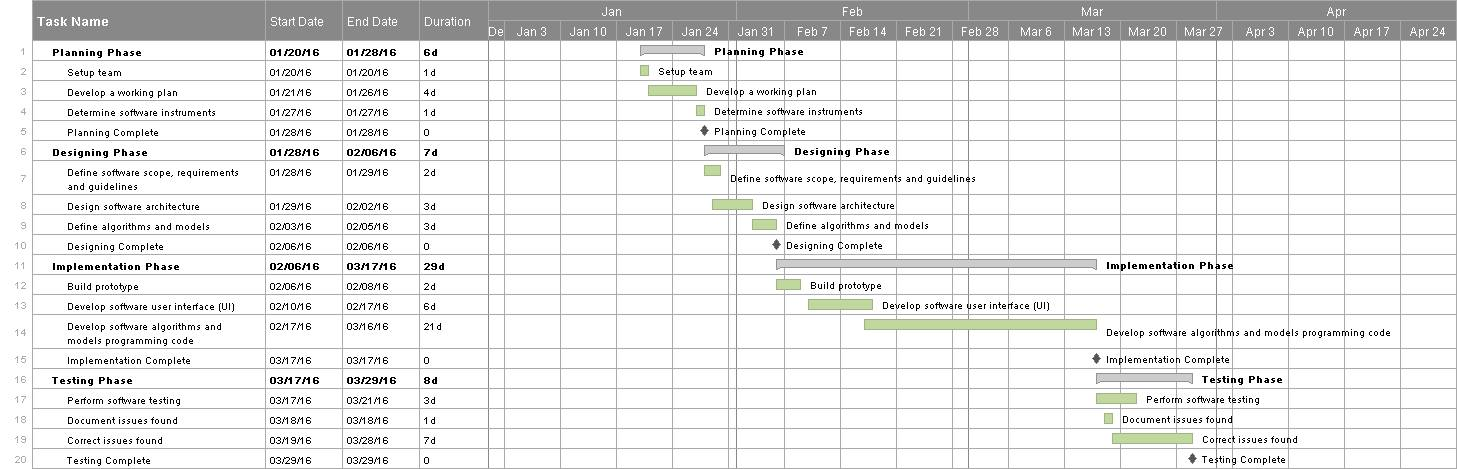
\includegraphics[scale=0.45, angle=90]{gantt}
\centering
\end{figure}